\documentclass[a4paper,twocolumn,11pt,accepted=2017-05-09]{quantumarticle}
\pdfoutput=1
\usepackage[utf8]{inputenc}
\usepackage[english]{babel}
\usepackage[T1]{fontenc}
\usepackage{amsmath}
\usepackage{hyperref}

\usepackage{tikz}
\usepackage{lipsum}
\usepackage{graphicx}

\usepackage{mathtools}
\DeclarePairedDelimiter\bra{\langle}{\rvert}
\DeclarePairedDelimiter\ket{\lvert}{\rangle}
\DeclarePairedDelimiterX\braket[2]{\langle}{\rangle}{#1 \delimsize\vert #2}

\begin{document}

\title{Qurry: A prototype quantum programming language}

\author{Lucas~Saldyt}
\affiliation{Arizona State University}
\email{lsaldyt@asu.edu}
\homepage{https://github.com/LSaldyt}
\maketitle

\begin{abstract}
    Innovation in near-term quantum programming requires the use of lightweight, transparent abstraction mechanisms.
    This paper outlines a typeless, dynamic functional quantum programming language, and a surrounding software system which allows for rapid prototyping and evolution of the langauge.
    Abstractions are desirable because they allow a programmer to express more computation with less code.
    Transparency is crucial, especially in quantum computing, because hardware details more strongly affect the types of programs that can be written.
    To some extent, abstraction and transparency oppose one another.
    However, carefully crafted abstractions can be lightweight enough to preserve transparency.
    Qurry achieves lightweight abstractions through heirarchical composition of data and of operations.
\end{abstract}

\section{Introduction}

Currently, quantum programming is analogically in a similar stage to classical programming in 1960s and early 1970s. 
A true high-level quantum programming language is still a desideratum.
In the history of classical programming languages, C, while not perfect, filled a major gap that had existed before its time \cite{kernighan2006c}, and quantum computing still lacks a similar language.
Importantly, C's evolution was partially driven by the need for a language expressive enough to easily re-code Unix.
Quantum languages, of course, are driven by a different motivation, primarily the power that quantum computing adds to the existing classical computing stack.
Importantly, quantum programming does not appear to be replacing classical computation, but adding to it.
Often quantum computers are used as auxillary elements to classical computers in hybrid computation.
According to the needs of the field, a high-level quantum programming language will likely need to be lightweight, hybridized, and transparent. While myriad other desirable criteria exist, these are certainly among them.

Hybridized instruction languages already exist, and allow one to leverage the power of existing classical computation \cite{forest, cirq, qasm, pyquil}.
However, the ability to program at a higher level of abstraction is desired.
It is not that it is particularly hard to write quantum circuits at the gate-level, but simply that existing quantum programming languages often force programmers to write redundant inexpressive code, in the sense that more description is required to get the same level of computation.
An obstruction to this is that running circuits on quantum hardware is not trivial, and requires transparency in a given language.

In the design philosophy of C++, Bjarne Stroustrup describes ``lightweight abstractions“, which allow users to easily exploit the full power of their computer without having to write hand optimized assembly code \cite{stroustrup}:
``The aim [of C++] is to allow a programmer to work at the highest feasible level of abstraction by providing a simple and direct mapping to hardware and zero-overhead abstraction mechanisms"

However, some have argued for the importance of hardware, as in Google's phrase ``hardware aware, not hardware agnostic" \cite{google_cloud}.
Many aspects of hardware are particularly important, for instance, topology, which will potentially result in a programmer needing to modify a quantum algorithm for it to run on two separate computers.
Additionally, the error generation of a quantum computer is actually a crucial detail, even though quantum programmers might desire to ignore it.
In the current state of quantum computing, many details of hardware cannot yet be ignored. 
However, it is obvious that \emph{eventual} hardware independence is desirable --- Consider the power of Java in the classical computing world. Lightweight abstractions are precisely the scaffold that will catalyze this transition.

In 1981, Richard Feynman noted that quantum physics appears to be impossible to simulate using a classical computer, but that quantum computers appeared to be perfectly capable of simulating quantum physics \cite{feynman_1981}.

Effectively, quantum computation potentially allows new problems to be computed efficiently: in particular, this includes literal simulations of the physical world, but also abstract algorithms which may receive a superpolynomial change in time complexity.
Qurry allows quantum programmers to access the power of quantum computers, without sacrificing performance or understanding of the underlying mechanisms.
\cite{nc}

\cite{larose2019overview}

\cite{selinger2006lambda}
\cite{selinger2004towards}


\cite{quipper}
\cite{quipper_guide}
\cite{proto_quipper}


\cite{omer1998procedural}
\cite{biamonte2017quantum}

\cite{lloyd2006programming}
\cite{hickey2008clojure}

\subsection{Motivation}

Stephen Jordan, of Microsoft, keeps a nearly exhaustive list of quantum algorithms and the speedups that they offer \cite{jordan}.
According to this list at time of writing, there are thirty-five distinct quantum algorithms which offer a potential superpolynomial speedup.
This famously includes Peter Shor's factoring and discrete log algorithms, as well as, fundamentally, quantum simulation.
\cite{shor, small_molecule_sim, feynman, lanyon2010towards}
Interestingly, many quantum algorithms such as the Deutsch-Jozsa algorithm are matched (at least practically, and sometimes theoretically) by probabilistic algorithms, and even some algorithms with superpolynomial speedups are based on older probabilistic versions.  \cite{deutsch1992rapid}
For instance, machine learning does not appear to have superpolynomial improvements at time of writing.
The most promising application of quantum computing in the near term is in molecular simulation.
As the comparisons section will demonstrate, Qurry offers unique programming language features which implementing each of these algorithms significantly easier.

% At time of writing, quantum computers have been used to simulate di-Hydrogen, Be-H2, and [Other small molecules, Cite]
% [Qurry aims to assist in the development and implementation of each of these algorithms...]
% 
% Quantum computing [motivations]
% [TODO: General motivations, cite Rigetti, cite Haskell/LISP/Rich Hickey, cite Probabilistic programming languages]

\subsection{Background}

The absolute basics of quantum computing are not nearly as intimidating as they are sometimes made out to be.
The main requirement is linear algebra, but complex numbers and probability are also helpful. 
Conventionally, quantum data is represented on qubits.
When measured, qubits will be in *either* of two states: $\ket{0}$ or $\ket{1}$.
However, more generally, qubits are in a combination of these two states, which is known as a superposition.
A particular active qubit's state is described by two complex numbers, $\alpha$ and $\beta$, which are collected in a vector.
This is written in the simple equation: $$\ket{\psi} = \alpha\ket{0} + \beta\ket{1}$$.
However, the state vector $\alpha, \beta$ is not directly examinable.
Instead, when a qubit is measured, one measures $\ket{0}$ with probability $|\alpha|^2$, and $1$ with probability $|\beta|^2$, which must sum to $\ket{1}$.
For single qubits, a state is evolved in the model simply by multiplying the state vector for a qubit by a $2$ by $2$ unitary matrix, known as a one-qubit gate. This is written as $Av$.

For $n$ qubits, the state is simply a complex vector of length $2^n$, and a $n$ qubit gate is a $2^n \text{ by } 2^n$ matrix:
$$\ket{\psi} = \alpha_i\ket{s_i} \text{ for } s_i \in \{\{0, 1\}^n\}, 0 < i < 2^n - 1$$.
Once a given $n$-qubit quantum state is measured, the outcome is a single bit-string, $s_i$, with probability $|\alpha_i|^2$.
If it is possible to repeat this measurement (by preparing the quantum state multiple times), then a collection of measurements is a multinomial distribution defined by the states $s_i$ and probabilities $\alpha_i$, but this distribution has $2^n$ states, and measuring a quantum state only gives a single sample.

Importantly, past a single qubit, quantum states can be entangled.
Two states are entangled when the measurement outcome of one qubit is correlated with the measurement outcome of other qubits.
The simplest, most famous example of this is the Bell states, also known as EPR pairs.
For instance, in one Bell state, two qubits are either measured both as $\ket{0}$, or both as $\ket{1}$ (even when measured independently), but there is no probability for them to differ.
This is the basis for all interesting quantum algorithms.

To summarize, superposition is the fundamental state model for quantum computers, but a given quantum state cannot be measured directly, only sampled once.
Then, entanglement allows the correlation of measurements, which is a crucial ingredient in any useful quantum algorithm. 
Any quantum program is simply a combination of linear operators which affect the superposition.
Given an initial state, conventionally the zero vector, a quantum program $P$ operates on the state vector, and then the vector is sampled, by measuring a subset of its qubits.
Importantly, a quantum program $P$ is itself a linear operator, potentially further composed of other linear operators.
The data in a quantum program, at this level of abstraction, will only ever be a vector of qubits, but at higher levels of abstraction, this vector can be subsectioned into semantic datatypes, no differently than how C++'s fundamental memory model is a sequence of bytes.

At the same time, in hybrid classical-quantum computation, classical control can setup, run, and measure the outcomes of quantum sub-programs.
In this way, some quantum program $P$ will be embedded in a hybrid program.

\subsection{Circuit Languages}

At time of writing, Rigetti pyquil contains the following quantum gates and operations:

Single qubit gates and operations:

\begin{itemize}
    \item RESET, I, X, Y, Z, H, S, T
\end{itemize}

Qubit gates taking an angle as the the parameter and qubit as the second:

\begin{itemize}
    \item RX, RY, RZ, PHASE
\end{itemize}

Swap operators, where each takes two qubits, and PSWAP takes an additional angle as a first argument:

\begin{itemize}
    \item SWAP, ISWAP, and PSWAP
\end{itemize}

Controlled operators:

\begin{itemize}
    \item CZ, CNOT %['control', 'target']
    \item CSWAP %['control', 'target\_1', 'target\_2']
    \item CPHASE00, CPHASE01, CPHASE10, CPHASE %['angle', 'control', 'target']
\end{itemize}

And of course the hybrid measurement instruction, which takes a qubit as the first argument, and a classical register as the second:

\begin{itemize}
    \item MEASURE
\end{itemize}

And also contains the following classical operations:

\begin{itemize}
    \item TRUE, FALSE, NOT, NEG %['classical\_reg']
    \item AND, OR, MOVE, EXCHANGE, IOR, XOR %['classical\_reg1', 'classical\_reg2']
    \item ADD, SUB, MUL, DIV %['classical\_reg', 'right']
    \item EQ, GT, GE, LE, LT %['classical\_reg1', 'classical\_reg2', 'classical\_reg3']
    \item LOAD %['target\_reg', 'region\_name', 'offset\_reg']
    \item STORE %['region\_name', 'offset\_reg', 'source']
    \item CONVERT %['classical\_reg1', 'classical\_reg2']
\end{itemize}

Most importantly, though, QUIL actually already has a notion of higher-level functions, which it calls ``Modifiers".
These are the following:
\begin{itemize}
    \item DAGGER
    \item CONTROLLED
\end{itemize}

\subsection{Classical Probabilistic Languages}

\cite{carpenter2017stan}
\cite{goodman2012church}

 Classical probabilistic programming languages are a recent innovation from the MIT cognitive science community. 
 Essentially, they create a way for non-expert programmers to access the power of Bayesian inference. 
 Users can create simple probabilistic models in standard code, and then run them through an expert-created inference backend.
 Famously, this has resulted in dramatically reduced code complexity, with a famous case where a 50-line probabilistic program could compete with traditional approaches to face recognition [TODO: Cite].

 Qurry is inspired by the effects these languages have had, and in fact there is some overlap between quantum programming and classical probabilistic languages.
 For instance, quantum bayesian inference has been conceptualized since the 70s-90s [Cite].
 %There are 10-billion cool libraries that use quantum bayesian inference [Cite].

\subsection{Parallels to C++ and its role in the classical software ecosystem}


\section{Features}

    Creating abstractions in quantum programming languages comes down to the creation of higher-order functions and higher-order datatypes.
    Language features that allow the creation and composition of both higher-order functions and higher-order datatypes set Qurry apart from lower-level circuit languages.

    \subsection{Higher Order Functions}

    The simplest illustration of a higher order function is trivial, but surprisingly neglected from any existing quantum language: it is the tensor operator ($U^{\otimes n}$), known to functional programmers as the higher-order function, \emph{map}.
    Many quantum algorithms will begin with a change of basis, effectively a state preparation. 
    Commonly, this is to the Hadamard basis, and is done by applying the Hadamard operator to a block of qubits.
    In a conventional circuit language, this is done as the following:
    \begin{verbatim}
    H 0
    H 1
    ...
    H n\end{verbatim}
    However, textbooks and papers will write this as $H^{\otimes n}$, and in Qurry, it can be written:
    \begin{verbatim}
    (define workspace (block n qubit))
    (map H workspace)\end{verbatim}
    Implicitly, this example also introduces Qurry's assignment statement \emph{define}, and its representation for qubit arrays, the $block$ command, which takes a size and a type, and allocates space and handles mapping to actual qubit indices.
    More impressively, Qurry supports automatic currying of functions:
    \begin{verbatim}
    (define initialize_basis (map H))
    (define workspace (block n qubit))
    (initialize_basis workspace)\end{verbatim}

    Of course, Qurry utilizes the two existing higher-order functions defined by QUIL: DAGGER, and more importantly, CONTROLLED.
    For brevity, Qurry redefines CONTROLLED to CU.
    Effectively, this allows the creation of arbitrary controlled operators, for instance the redefinition of CNOT:
    \begin{verbatim}
    (define custom_cnot (CU X))
    (H 0)
    (custom_cnot 0 1)
    \end{verbatim}
    Qurry calls functions like CU controlled higher level operators.
    This list includes:
    \begin{itemize}
        \item CU 
        \item CNU
        \item Cascade, CascadeU
        \item ReverseCascade, ReverseCascadeU
        \item Collect, CollectU
        \item Expand, ExpandU
        \item SimU
    \end{itemize}
    Interestingly, many of these are defined through composition of simpler gates.
    For instance, CNU takes a block of control qubits and a block of work qubits, and entangles pairs of control and work qubits, and finally entangles a target qubit, which a unitary is controlled by.
    Essentially, each of these operators performs some control operations (through a composition of CNOT gates, conventionally), and then performs an arbitrary unitary operation which is controlled by the result of the previous control operations.
    (This section will contain circuits and more in-depth explanations, but this is currently commented out).
    %[TODO: Circuit Diagram]
    %A ``Cascade" is simply a chain of shifted CNOT gates, and a ``CascadeU" is simply a ``Cascade" which in turn controls the operation of a unitary gate.
    %[Circuit Diagram]
    %ReverseCascade:
    %[Circuit Diagram]
    %Now consider the circuit used for the simulation of a hamiltonian ():
    %[Circuit Diagram]
    %Clearly, this circuit contains repeated information, which can be abstracted into the form of another function: ``SimU", which in turn is a "collect" operation, an "expand" operation, and a controlled unitary in between them.
    %[Circuit Diagram]

    Lastly, Qurry implements lambda expressions, which allow arbitrary re-use and composition of other operators, and natively support currying.
    Since the $\lambda$ character is unavailable on most conventional keyboards, lambda expressions are denoted with an $l$, and can be used to create named functions, such as:
    \begin{verbatim}
    (define create-bell (l (a b) ((H a) (CNOT a b))))
    \end{verbatim}
    And of course they support currying:
    \begin{verbatim}
    (define partial ((l (a b c) ((X a) (X b) (CCNOT a b c))) 0 1))
    (partial 2)
    \end{verbatim}
    Obviously, Qurry's lisp interface will have plenty of parentheses.

    \subsection{Higher Order Datatypes}

    Qurry's memory model is simple: an array of $n$ qubits, and $m$ classical bits.
    However, in programmer-space, these arrays are cut up and defined using semantic datatypes.

    The previous section discussed the \emph{block} type, and the \emph{define} command.
    The \emph{block} command will automatically select appropriate qubits in the array, and map to these when used.

    In terms of datatypes, not much more is needed, except for the \emph{datatype} command, which mimics C++'s \emph{struct} or \emph{class}.
    For simplicity, elegance, and robustness, Qurry does not implement encapsulation or inheritance, but instead uses public access by default (in the spirit of Python, since after all, Qurry has a Python interface), and relies on composition instead of inheritance.
    A \emph{datatype} is nothing more than a contiguous collection of other Qurry datatypes, with names for each field.
    Like \emph{block} objects, \emph{datatype}s automatically map to qubits and bits in Qurry's memory model.
    These can be \emph{block}s, single qubits, single bits, and other defined \emph{datatype} objects, allowing for recursive types.
    Fields within a datatype are simply accessed with the dot operator:
    % TODO: should functions be possible as datatype fields?
    \begin{verbatim}
        (datatype entanglion
                  (a qubit)
                  (b qubit))
        (define e (entanglion))
        (H e.a)
        (CNOT e.a e.b)
    \end{verbatim}

    Recursively composed higher-order datatypes, in combination with recursively composed higher-order functions are the foundation for creating a more abstract programming language.

    \subsection{Other Features}

    Lastly, Qurry features rudimentary classical features meant to complement the hybrid model used by QUIL.

    \begin{itemize}
        \item cond 	    
        \item do 	        
    \end{itemize}


 \section{Comparisons}
    This section is currently commented out.
% 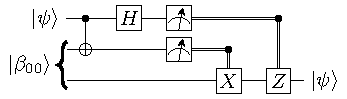
\includegraphics{teleport.pdf}
% 
%     Draw examples from Nielsen and Chuang, and the general literature.
% 
%  Simply change (if (condition) (branch) (branch))
%  into
%  ``
%  Condition
%  Measure []
%  Jump label
%  branch
%  branch etc
%  ``
%  
%  Curry also supports variable naming, blocks of qubits, classical callbacks, imports, \dots
%  Curry can be called as a library and operated from python
%  
%  There are some easy targets for providing abstraction: common things like functions, conditionals, loops, integer data types, and so on. 
%  However, let's jump into the quantum/probabilistic side of things.
%  
%  Models will fundamentally be composed of, generally, wave functions: Superpositions over all possible states.
%  First, consider modeling a classical distribution. 
%  We can successfully produce sampleable classical distributions on a quantum computer.
%  For instance, consider the following model from the Church programming language tutorial.
%  This code is specifying a probabilistic grammar for simple sentences about cooking.
%  
%  ```scheme
%  (define (transition nonterminal)
%    (case nonterminal
%          (('D) (multinomial(list (list (terminal 'the))
%                                  (list (terminal 'a)))
%                            (list (/ 1 2) (/ 1 2))))
%          (('N) (multinomial (list (list (terminal 'chef))
%                                   (list (terminal 'soup))
%                                   (list (terminal 'omelet)))
%                             (list (/ 1 3) (/ 1 3) (/ 1 3))))
%          (('V) (multinomial (list (list (terminal 'cooks))
%                                   (list (terminal 'works)))
%                             (list (/ 1 2) (/ 1 2))))
%          (('A) (multinomial (list (list (terminal 'diligently)))
%                             (list (/ 1 1))))
%          (('AP) (multinomial (list (list 'A))
%                              (list (/ 1 1))))
%          (('NP) (multinomial (list (list 'D 'N))
%                              (list (/ 1 1))))
%          (('VP) (multinomial (list (list 'V 'AP)
%                                    (list 'V 'NP))
%                              (list (/ 1 2) (/ 1 2))))
%          (('S) (multinomial (list (list 'NP 'VP))
%                             (list (/ 1 1))))
%          (else 'error)))
%  ```
%  
%  More succinctly, this is specifying the following (toy) language model:
%  ```scheme
%  D(eterminer):      (uniform 'the' 'a')
%  N(oun):            (uniform 'chef' 'omelet' 'soup')
%  V(erb):            (uniform 'cooks' 'works')
%  A(dverb):          (uniform 'diligently')
%  AP(Adverb Phrase): (uniform A)
%  NP(Noun Phrase):   (D, N)
%  VP(Verb Phrase):   (uniform (V AP) (V NP))
%  S(entence):        (NP, VP)
%  ```
%  
%  To make things even simpler, let's first just consider modeling a randomly sampled Noun-Phrase (which is the first part in sampling a full toy sentence).
%  The noun-phrase is a concatenation of a determiner and a noun. In our toy example, we have two determiners and three nouns, both uniformly sampled, which makes for a total of six options with equal probability.
%  So, we'll need three qubits to model this. Curry has builtins for these distributions.
%  ```scheme
%  (def determiner-qubit 0)
%  (def noun-qubits 1 2)
%  (bernoulli 0.5 determiner-qubit)
%  (multinomial 0.33 0.33 0.34 noun-qubits)
%  ```
%  
%  The output is the following (using a local simulator):
%  ```
%  grid {curry}: ./compile examples/test.lisp
%  
%  [['def', 'determiner-qubit', '0'],
%   ['def', 'noun-qubits', '1', '2'],
%   ['bernoulli', '0.5', 'determiner-qubit'],
%   ['multinomial', '0.33', '0.33', '0.34', 'noun-qubits']]
%  
%  {'000': 0.17, '001': 0.16, '010': 0.17, '011': 0.17, '100': 0.16, '101': 0.16}
%  
%  277.4035930633545 ms simulated runtime
%  ```
%  
%  In our output, the rightmost bit is representing the determiner, and the other two bits are representing the noun.
%  So the output is:
%  ```python3
%  {'the chef' : 1/6, 'a chef' : 1/6, 'the omelet' : 1/6, 'a omelet' : 1/6, 'the soup' : 1/6, 'a soup' : 1/6}
%  ```
%  Now, let's consider the rest of the model.
%  When we sample a Verb Phrase, it contains recursive elements.
%  So, it will branch (with equal probabilities) to either (V AP) or (V NP).
%  Before diving in, let's look at branching in quantum computers.
%  
%  Consider preparing a bell state:
%  ```
%  (h 0)
%  (cnot 0 1)
%  ```
%  And distinguish this from the following, which will produce the same classical measurements, but no entanglement (because the state of the first qubit is known before producing the state in the second qubit). 
%  In this case, the state 01 is possible, because the first qubit may be measured in the 1 state, and the second qubit is unprepared, and in the zero state.
%  ```
%  (bernoulli 0.5 0)
%  (measure 0 0)
%  (if 0 (x 1) (nop))
%  ```
%  
%  So, when creating a probabilistic model which branches, we distinguish between these two types of branching, because only one truly creates an entangled state.
%  However, this makes representing information slightly more difficult, because we will not know which bits correspond to which states (unless we encode this, which we will).

\section{Software Ecosystem}

In addition to being a prototype quantum programming language, Qurry defines a software stack surrounding the language, which is intended to make development more pleasant.
For instance, this software stack makes it exceptionally easy to add new language features and libraries to Qurry.
This allows one to rapidly test new ideas in quantum programming and let the language evolve on its own as opposed to architecting a top-down ``perfect'' language.

\section{Standard Library}

    Qurry contains mechanisms which enable easy inclusion of qurry code in the form of libraries.
    As an example, Qurry's standard library is implemented in this fashion.

    Explain how the statistics library can be easily implemented.

    At time of writing, Qurry contains the following constructs:  	
    \begin{itemize}
	    \item gaussian 	
        \item bernoulli
	    \item multinomial 	
	    \item uniform
    \end{itemize}

    Similarly to in a classical probabilistic programming language, these enable the creation of classical probabilistic states, which can then be used in quantum programs.
    For instance, it is possible to create a multi-dimensional gaussian distribution, and then entangle an auxillary qubit with the state of the gaussian distribution.

    \section{Extension}

    Making additions to Qurry is particularly easy:
    For instance, the $map$ feature is defined using the following python code:

    \begin{verbatim}
from ..compiler.utils import named_uuid

def map(operator, blockname, kernel=None):
    '''
    Apply a single-qubit operator to every qubit in a block
    (map H blocka)
    '''
    try:
        block = kernel.definitions[blockname]
    except KeyError:
        raise ValueError('The block {} is not defined'.format(blockname))
    return '\n'.join('{} {}'.format(operator, i)
            for i in range(block.start, block.end + 1))
    \end{verbatim}

\section{Statistical Libraries}

Since quantum computers are simply special probabilistic computers, Qurry also attempts to create a classical statistical library for high-level modeling. 
This is particularly useful in the same way that a classical probabilistic programming language is, namely for modeling anything statistical, and especially for bayesian machine learning.
For instance, the R. Tucci and H. Dekant's group have shown uses for this through their software, Bayesforge [TODO: Cite].
Qurry includes simple statistical packages for creating states, but no inference engine.
[However, Qurry might allow one to interface with Bayesforge]

\section{Conclusion}

In the creation of a Qurry and its corresponding framework, it is hoped that this will aid the development of quantum algorithms, as algorithm designers will have a new, richer, more abstract vocabulary with which to express themselves.
To recap, this goal is approached in the following N ways.
By introduction of lightweight abstractions from the C++ school of thought, efficient and transparent programming interfaces are created.
Through specialized libraries, Qurry can claim to be a generalized library, while still offering powerful sub-frameworks for specific tasks.
With functional programming paradigms, Qurry can move towards higher levels of abstraction as the semantics of quantum programming become better understood.
Lastly, by creating a rapid prototyping framework, new language features can be developed in a bottom-up style, which will allow Qurry to be created naturally, instead of artificially.

 \section{Appendix one}
Appendix content

\section*{Acknowledgment}

The author would like to thank Dr. Will Zeng of Rigetti computing, an organizer of the Unitary Fund, Dr. Ajay Bansal of Arizona State University, PLoS and other donators to the unitary fund, and ASU's FURI program.

\newpage

\bibliographystyle{unsrt}
\bibliography{sources}

 % \begin{abstract}
 %   In the standard, \texttt{twocolumn}, layout the abstract is typeset as a bold face first paragraph.
 %   Quantum also supports a \texttt{onecolumn} layout with the abstract above the text.
 %   Both can be combined with the \texttt{titlepage} option to obtain a format with dedicated title and abstract pages that are not included in the page count.
 %   This format can be more suitable for long articles.
 %   The \texttt{abstract} environment can appear both before and after the \texttt{\textbackslash{}maketitle} command and calling \texttt{\textbackslash{}maketitle} is optional, as long as there is an \texttt{abstract}.
 %   Both \texttt{abstract} and \texttt{\textbackslash{}maketitle} however must be placed after all other \texttt{\textbackslash{}author}, \texttt{\textbackslash{}affiliation}, etc.\ commands, see also Section~\ref{sec:title-information}.
 %   If you provide the ORCID number of an author by using the \texttt{\textbackslash{}orcid} command, the author name becomes a link to their page on \href{http://orcid.org/}{orcid.org}. 
 % \end{abstract}
 % 
 % In the \texttt{twocolumn} layout and without the \texttt{titlepage} option a paragraph without a previous section title may directly follow the abstract.
 % In \texttt{onecolumn} format or with a dedicated \texttt{titlepage}, this should be avoided.
 % 
 % Note that clicking the title performs a search for that title on \href{http://quantum-journal.org}{quantum-journal.org}.
 % In this way readers can easily verify whether a work using the \texttt{quantumarticle} class was actually published in Quantum.
 % If you would like to use \texttt{quantumarticle} for manuscripts not yet accepted in Quantum, or not even intended for submission to Quantum, please use the \texttt{unpublished} option to switch off all Quantum related branding and the hyperlink in the title.
 % By default, this class also performs various checks to make sure the manuscript will compile well on the arXiv.
 % If you do not intend to submit your manuscript to Quantum or the arXiv, you can switch off these checks with the \texttt{noarxiv} option.
 % On the contrary, by giving the \texttt{accepted=YYYY-MM-DD} option, with \texttt{YYYY-MM-DD} the acceptance date, the note ``Accepted in Quantum YYYY-MM-DD, click title to verify'' can be added to the bottom of each page to clearly mark works that have been accepted in Quantum. 
 % 
 % \section{Figures}
 % \begin{figure}[t]
 %   \centering
 %   \includegraphics{example-plot.pdf}
 %   \caption{Every figure must have an informative caption and a number.
 %     The caption can be placed above, below, or to the side of the figure, as you see fit.
 %     The same applies for tables, boxes, and other floating elements. 
 %     Quantum provides a Jupyter notebook to create plots that integrate seamlessly with \texttt{quantumarticle}, described in Section \ref{sec:plots}.
 %     Figures spanning multiple columns can by typeset with the usual \texttt{figure*} environment.}
 %   \label{fig:figure1}
 % \end{figure}
 % See Fig.~\ref{fig:figure1} for an example of how to include figures.
 % Feel free to place them at the top or bottom of the page, or in the middle of a paragraph as you see fit.
 % Try to place them on the same page as the text referring to them.
 % A figure on the first page can help readers remember and recognize your work more easily.
 % 
 % \section{Sectioning and equations}
 % Sections, subsections, subsubsections, and paragraphs should be typeset with the standard LaTeX commands.
 % You can use the standard commands for equations.
 % \begin{align}
 %   \label{emc}
 %   E &= m\,c^2\\
 %   a^2 + b^2 &= c^2\\
 %   H\,|\psi\rangle &= E\,|\psi\rangle\\
 %   (\openone \otimes A)\,(B \otimes \openone) &= A \otimes B
 % \end{align}
 % For multi-line equations \texttt{align} is \href{http://tex.stackexchange.com/questions/196/eqnarray-vs-align}{preferable} over \texttt{eqnarray}.
 % Please refrain from using the latter.
 % For complex equations you may want to consider using the \texttt{IEEEeqnarray} environment from the \texttt{IEEEtrantools} package.
 % Whether you prefer to refer to equations as Eq.~\eqref{emc}, Equation~\ref{emc}, or just \eqref{emc} is up to you, but please be consistent and use the \texttt{\textbackslash{}eqref\{\dots\}} command instead of writing \texttt{(\textbackslash{}ref\{\dots\})}.
 % As a courtesy for your readers and referees, please suppress equation numbers only if there is a specific reason to do so, to not make it unnecessarily difficult to refer to individual results and steps in derivations.
 % 
 % \paragraph{Paragraphs}
 % The paragraph is the smallest unit of sectioning.
 % Feel free to end the paragraph title with a full stop if you find this appropriate.
 % 
 % \subsection{References and footnotes}
 % \label{sec:subsec1}
 % Footnotes\footnote{Only use footnotes when appropriate.} appear in the bottom of the page.
 % Please do not mix them with your references.
 % 
 % Citations to other works should appear in the References section at the end of the work.
 % 
 % \begin{theorem}[DOI links are required]
 %   Important: As Quantum is a member of Crossref, all references to works that have a DOI must be hyperlinked according to the DOI. Those links must start with \texttt{https://doi.org/} (preferred), or \texttt{http://dx.doi.org/}. Direct links to the website of the publisher are not sufficient.
 % \end{theorem}
 % 
 % This can be achieved in several ways, depending on how you are formatting your bibliography.
 % Suppose the DOI of an article \cite{examplecitation} that you want to cite is \texttt{10.22331/idonotexist}.
 % If you are formatting your bibliography manually, you can cite this work using the following in your \texttt{thebibliography} environment:
 % \begin{verbatim}
 % \bibitem{examplecitation}
 %   Name Surname,
 %   \href{https://doi.org/10.22331/
 %         idonotexist}{Quantum
 %         \textbf{123}, 123456 (1916).}
 % \end{verbatim}
 % 
 % \begin{theorem}[One citation per bibitem]
 %   Important: If you are formatting your bibliography manually, please do not group multiple citations into one \texttt{\textbackslash{}bibitem}.
 %   Having to search through multiple references to find the cited result makes your work less accessible for authors and grouping references can screw up our automatic extraction of citations.
 % \end{theorem}
 % 
 % We encourage the use of BibTeX to generate your bibliography from the BibTeX meta-data provided by publishers.
 % For DOI linking to work, the BibTeX file must contain the \texttt{doi} field as for example in:
 % \begin{verbatim}
 % @article{examplecitation,
 %   author = {Surname, Name},
 %   title = {Title},
 %   journal = {Quantum},
 %   volume = {123},
 %   page = {123456},
 %   year = {1916},
 %   doi = {10.22331/idonotexist},
 % }
 % \end{verbatim}
 % Several authors had problems because of Unicode characters in their BibTeX files.
 % Be advised that \href{http://wiki.lyx.org/BibTeX/Tips}{BibTeX does not support Unicode characters}.
 % All special characters must be input via their respective LaTeX commands.
 % 
 % If you are using BibTeX, you can load the \texttt{natbib} package by putting
 % \begin{verbatim}
 % \usepackage[numbers,sort&compress]{natbib}
 % \end{verbatim}
 % in the preamble of your document and then use the \texttt{plainnat} citation style by including your BibTeX bibliography \texttt{mybibliography.bib} where you want the bibliography to appear as follows:
 % \begin{verbatim}
 % \bibliographystyle{plainnat}
 % \bibliography{mybibliography}
 % \end{verbatim}
 % The quantumarticle class automatically detects that the \texttt{natbib} package was loaded and redefines the \texttt{\textbackslash{}doi} command to create hyperlinks.
 % This is likely the easiest option if you are converting from another document class.
 % 
 % If you want to use BibLaTeX, you can instead add
 % \begin{verbatim}
 % \usepackage[backend=bibtex]{biblatex}
 % \addbibresource{mybibliography.bib}
 % \end{verbatim}
 % to the preamble of your document and then output the bibliography with
 % \begin{verbatim}
 % \printbibliography
 % \end{verbatim}
 % where appropriate.
 % You then have to upload the .bbl file along with the other source files when submitting to the arXiv.
 % Due to incompatibilities between different BibLaTeX versions we unfortunately cannot recommend this option \cite{biblatexsubmittingtothearxiv}.
 % 
 % The quantumarticle class automatically detects that the \texttt{biblatex} package was loaded, sets the default option \texttt{doi=true} to include the DOI in the bibliography, and declares a suitable field format to make it a hyperlink.
 % Due to issues with \texttt{biber} we recommend to use the \texttt{bibtex} backend of \texttt{biblatex}.
 % 
 % More information on how to get DOI links in your document can be found on StackExchange \cite{howtogetdoilinksinbibliography,automaticallyaddingdoifieldstoahandmadebibliography}.
 % Feel free to change the appearance of citations in any way you like by using a different \texttt{bibliographystyle} or via the advanced mechanisms provided by BibLaTeX.
 % The only two requirements are that citations must uniquely identify the cited work and that they must contain a DOI hyperlink whenever possible.
 % 
 % \begin{theorem}[Use \texttt{\textbackslash pdfoutput=1}]
 %   In order to get correct line breaks within hyperlinks and to make sure the arXiv produces a PDF as output, please add the line 
 % \begin{verbatim}
 % \pdfoutput=1
 % \end{verbatim}
 %   within the first 5 lines of your main LaTeX file, as suggested by the arXiv \cite{arxivpdfoutput}.
 % \end{theorem}
 % 
 % \section{Plots}
 % \label{sec:plots}
 % Quantum provides a \href{https://jupyter.org/}{Jupyter notebook} based on the widely used \href{https://matplotlib.org/}{matplotlib} library that greatly simplifies the creation of plots that integrate seamlessly with the \texttt{quantumarticle} document class. This is intended as a service to the authors, is \textit{not} mandatory, and currently in beta stage. You can download the \href{https://raw.githubusercontent.com/quantum-journal/quantum-journal/master/quantum-plots.ipynb}{quantum-plots.ipynb} notebook and accompanying \href{https://raw.githubusercontent.com/quantum-journal/quantum-journal/master/quantum-plots.mplstyle}{quantum-plots.mplstyle} file from the \href{https://github.com/quantum-journal/quantum-journal}{quantumarticle GitHub repository}. You only need to specify the font size and paper format that were passed as options to \texttt{quantumarticle} to get plots with fitting font sizes and dimensions.
 % We strongly encourage authors to use the vector based PDF format for plots.
 % 
 % \begin{theorem}[Be mindful of the colorblind]
 %   About 4\% of the worlds population are affected by some form of color vision deficiency or color blindness.
 %   Please make sure that your plots and figures can still be understood when printed in gray scale and avoid the simultaneous use of red and green, as the inability to distinguish these two colors is the most widespread form of color vision deficiency.
 % \end{theorem}
 % 
 % \section{Summary section}
 % Longer articles should include a section that, early on, explains the main results, their limitations, and assumptions.
 % This section can be used to, for example, present the main theorem, or provide a summary of the results for a wider audience.
 % 
 % \section{Extra packages}
 % Quantum encourages you to load the following extra packages:
 % \begin{verbatim}
 % \usepackage[utf8]{inputenc}
 % \usepackage[english]{babel}
 % \usepackage[T1]{fontenc}
 % \usepackage{amsmath}
 % \usepackage{hyperref}
 % \end{verbatim}
 % If you do not load the \texttt{hyperref} package, quantumarticle automatically loads it for you.
 % Packages that change font settings, such as \texttt{times} or \texttt{helvet} should be avoided.
 % 
 % \section{Wide equations}
 % Very wide equations can be shown expanding over both columns using the \texttt{widetext} environment.
 % In \texttt{onecolumn} mode, the \texttt{widetext} environment has no effect.
 % \begin{widetext}
 %   \begin{equation}
 % |\mathrm{AME}(n=6,q=5)\rangle=\sum_{i,j,k=0}^4 |i,j,k,i+j+k,i+2j+3k,i+3j+4k\rangle
 %   \end{equation}
 % \end{widetext}
 % To enable this feature in \texttt{twocolumn} mode, \texttt{quantumarticle} relies on the package \texttt{ltxgrid}.
 % Unfortunately this package has a bug that leads to a sub-optimal placement of extremely long footnotes.
 % 
 % \section{Title information}
 % \label{sec:title-information}
 % You can provide information on authors and affiliations in the common format also used by \texttt{revtex}:
 % \begin{verbatim}
 % \title{Title}
 % \author{Author 1}
 % \author{Author 2}
 % \affiliation{Affiliation 1}
 % \author{Author 3}
 % \affiliation{Affiliation 2}
 % \author{Author 4}
 % \affiliation{Affiliation 1}
 % \affiliation{Affiliation 3}
 % \end{verbatim}
 % In this example affiliation 1 will be associated with authors 1, 2, and 4, affiliation 2 with author 3 and affiliation 3 with author 4.
 % Repeated affiliations are automatically recognized and typeset in \texttt{superscriptaddress} style.
 % Alternatively you can use a format similar to that of the \texttt{authblk} package and the \texttt{elsarticle} document class to specify the same affiliation relations as follows:
 % \begin{verbatim}
 % \title{Title}
 % \author[1]{Author 1}
 % \author[1]{Author 2}
 % \author[2]{Author 3}
 % \author[1,3]{Author 4}
 % \affil[1]{Affiliation 1}
 % \affil[2]{Affiliation 1}
 % \affil[3]{Affiliation 1}
 % \end{verbatim}
 % 
 % \section{LyX layout}
 % \label{sec:lyx-layout}
 % 
 % The quantumarticle document class comes bundled with a \href{https://raw.githubusercontent.com/quantum-journal/quantum-journal/master/quantum-lyx-template.lyx}{LyX layout} that allows to typeset manuscripts with the LyX document processor instead of directly writing LaTeX code. Please be aware that this is a beta feature that might not receive the same level of support as the quantumarticle document class itself.   
 % 
 % \section{Version}
 % \label{sec:version}
 % This is quantumarticle version v\quantumarticleversion.
 % 
 % \bibliographystyle{plain}
 % \begin{thebibliography}{9}
 % \bibitem{examplecitation}
 %   Name Surname,
 %   \href{https://doi.org/10.22331/
 %         idonotexist}{Quantum
 %         \textbf{123}, 123456 (1916).}
 % 
 % \bibitem{biblatexsubmittingtothearxiv}
 %   StackExchange discussion on \href{http://tex.stackexchange.com/questions/26990/biblatex-submitting-to-the-arxiv}{``Biblatex: submitting to the arXiv'' (2017-01-10)}
 % 
 % \bibitem{arxivpdfoutput}
 %   Help article published by the arXiv on \href{https://arxiv.org/help/submit_tex}{``Considerations for TeX Submissions'' (2017-01-10)}
 % 
 % \bibitem{howtogetdoilinksinbibliography}
 %   StackExchange discussion on \href{http://tex.stackexchange.com/questions/3802/how-to-get-doi-links-in-bibliography}{``How to get DOI links in bibliography'' (2016-11-18)}
 %   
 % \bibitem{automaticallyaddingdoifieldstoahandmadebibliography}
 %   StackExchange discussion on \href{http://tex.stackexchange.com/questions/6810/automatically-adding-doi-fields-to-a-hand-made-bibliography}{``Automatically adding DOI fields to a hand-made bibliography'' (2016-11-18)}
 % \end{thebibliography}
 % 
 % 
 % 
 % \onecolumn\newpage
 % \appendix
 % 
 % \section{First section of the appendix}
 % Quantum allows the usage of appendices.
 % 
 % \subsection{Subsection}
 % Ideally, the command \texttt{\textbackslash{}appendix} should be put before the appendices to get appropriate section numbering.
 % The appendices are then numbered alphabetically, with numeric (sub)subsection numbering.
 % Equations continue to be numbered sequentially.
 % \begin{equation}
 %   A \neq B
 % \end{equation}
 % You are free to change this in case it is more appropriate for your article, but a consistent and unambiguous numbering of sections and equations must be ensured.
 % 
 % If you want your appendices to appear in \texttt{onecolumn} mode but the rest of the document in \texttt{twocolumn} mode, you can insert the command \texttt{\textbackslash{}onecolumn\textbackslash{}newpage} before \texttt{\textbackslash{}appendix}.   
 % 
 % \section{Problems and Bugs}
 % In case you encounter problems using the quantumarticle class please analyze the error message carefully and look for help online; \href{http://tex.stackexchange.com/}{http://tex.stackexchange.com/} is an excellent resource.
 % If you cannot resolve a problem, please open a bug report in our bug-tracker under \href{https://github.com/quantum-journal/quantum-journal/issues}{https://github.com/quantum-journal/quantum-journal/issues}.
 % You can also contact us via email under \href{mailto:latex@quantum-journal.org}{latex@quantum-journal.org}, but it may take significantly longer to get a response.
 % In any case, we need the full source of a document that produces the problem and the log file showing the error to help you.
 % 
\end{document}
